\documentclass[tikz,border=10pt]{standalone}
\usepackage{mathabx}
\usetikzlibrary{backgrounds}
\usepackage{newunicodechar}
\newunicodechar{♮}{$\natural$}
\newunicodechar{♭}{$\flat$}
\newunicodechar{♯}{$\sharp$}
\newunicodechar{➚}{$\nearrow$}
\newunicodechar{➘}{$\searrow$}
\newunicodechar{Ȧ}{\stackon[0.8pt]{A}{.}}
\newunicodechar{Ḃ}{\stackon[0.8pt]{B}{.}}
\newunicodechar{Ċ}{\stackon[0.8pt]{C}{.}}
\newunicodechar{Ḋ}{\stackon[0.8pt]{D}{.}}
\newunicodechar{Ė}{\stackon[0.8pt]{E}{.}}
\newunicodechar{Ḟ}{\stackon[0.8pt]{F}{.}}
\newunicodechar{Ġ}{\stackon[0.8pt]{G}{.}}


\def\centerarc[#1](#2)(#3:#4:#5);%
{
  \draw[#1]([shift=(#3:#5)]#2) arc (#3:#4:#5);
}


\begin{document}
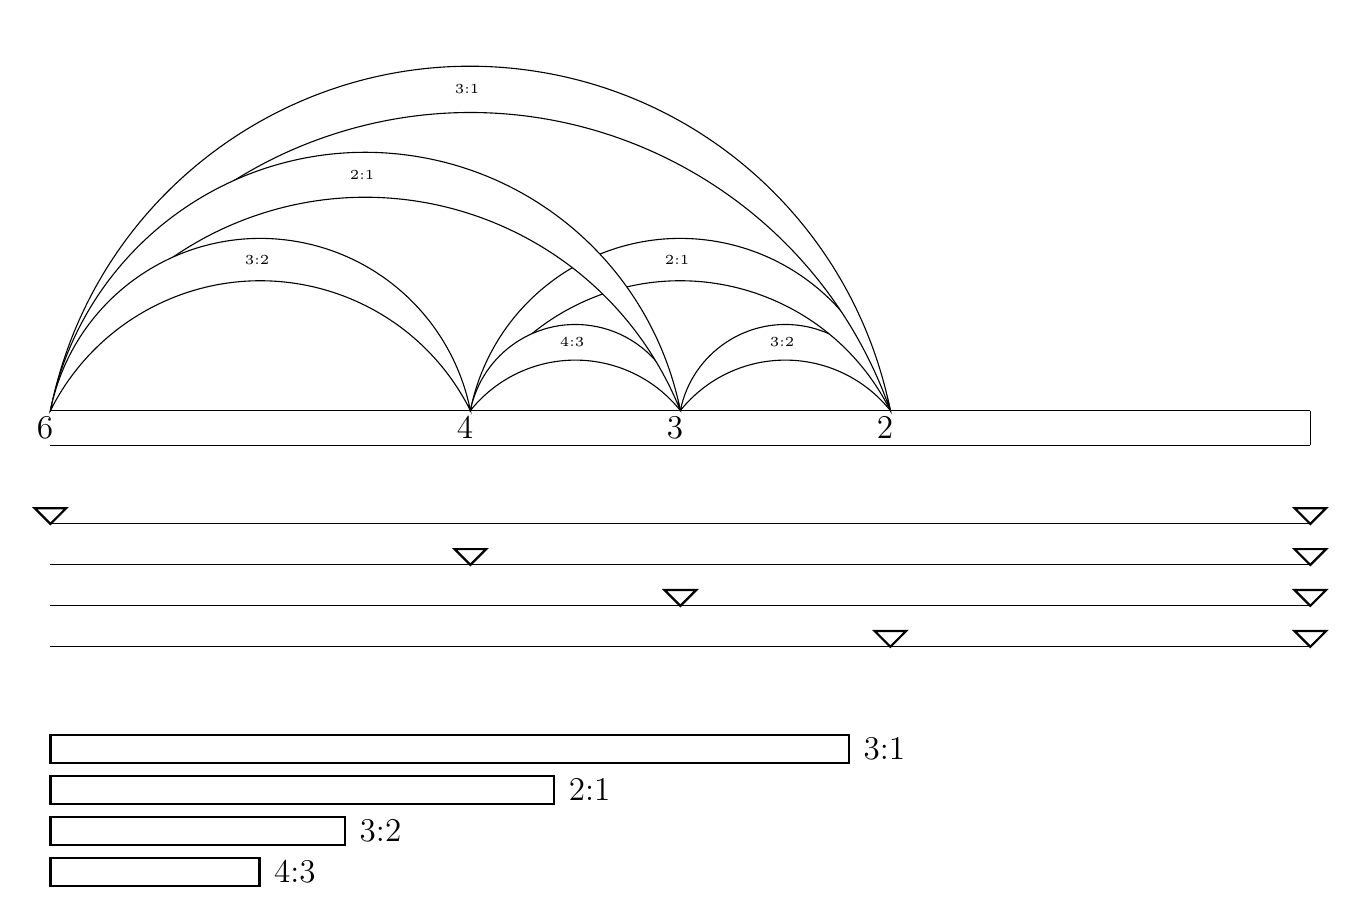
\begin{tikzpicture}

\draw (0.0,0.0) -- (16.0,0.0);
\draw (0.0,-0.44000003) -- (16.0,-0.44000003);
\draw (16.0,-0.44000003) -- (16.0,0.0);
\draw[fill=white] (8.0,0.0) arc[start angle=168.6900732010243, end angle=11.30993351547934, radius=1.3597387] arc[start angle=38.65980985328305, end angle=141.34020881605164, radius=1.7074999] -- cycle;
\node[align=center] at (9.333334,0.86695254) { \tiny 3:2 };
\draw[fill=white] (5.3333335,0.0) arc[start angle=168.69007234725063, end angle=11.309932661705695, radius=2.7194772] arc[start angle=26.56505088990245, end angle=153.43494045867556, radius=2.981424] -- cycle;
\node[align=center] at (8.0,1.9171174) { \tiny 2:1 };
\draw[fill=white] (5.3333335,0.0) arc[start angle=168.69007234725063, end angle=11.309932661705695, radius=1.3597385] arc[start angle=38.65980643818846, end angle=141.34018491038952, radius=1.7074997] -- cycle;
\node[align=center] at (6.666667,0.8669525) { \tiny 4:3 };
\draw[fill=white] (0.0,0.0) arc[start angle=168.69007234725063, end angle=11.309932661705695, radius=5.4389544] arc[start angle=19.29004565019262, end angle=160.70994569838535, radius=5.6505656] -- cycle;
\node[align=center] at (5.3333335,4.0780935) { \tiny 3:1 };
\draw[fill=white] (0.0,0.0) arc[start angle=168.6900732010243, end angle=11.30993351547934, radius=4.0792155] arc[start angle=21.80141058535793, end angle=158.19860808397675, radius=4.3081317] -- cycle;
\node[align=center] at (4.0,2.9936738) { \tiny 2:1 };
\draw[fill=white] (0.0,0.0) arc[start angle=168.69007234725063, end angle=11.309932661705695, radius=2.7194772] arc[start angle=26.56505088990245, end angle=153.43494045867556, radius=2.981424] -- cycle;
\node[align=center] at (2.6666667,1.9171174) { \tiny 3:2 };
\node[align=center] at (0.0, -0.22000001) { \large 6 };
\node[align=center] at (5.3333335, -0.22000001) { \large 4 };
\node[align=center] at (8.0, -0.22000001) { \large 3 };
\node[align=center] at (10.666667, -0.22000001) { \large 2 };
\draw (0.0,-1.4399999) -- (16.0,-1.4399999);
\draw[thick] (0.0, -1.4399999) -- (0.2, -1.24) -- (-0.2, -1.24) --  cycle;
\draw[thick] (16.0, -1.4399999) -- (16.2, -1.24) -- (15.8, -1.24) --  cycle;
\draw (0.0,-1.9599999) -- (16.0,-1.9599999);
\draw[thick] (5.3333335, -1.9599999) -- (5.5333333, -1.7599999) -- (5.133333, -1.7599999) --  cycle;
\draw[thick] (16.0, -1.9599999) -- (16.2, -1.7599999) -- (15.8, -1.7599999) --  cycle;
\draw (0.0,-2.48) -- (16.0,-2.48);
\draw[thick] (8.0, -2.48) -- (8.2, -2.28) -- (7.8, -2.28) --  cycle;
\draw[thick] (16.0, -2.48) -- (16.2, -2.28) -- (15.8, -2.28) --  cycle;
\draw (0.0,-3.0) -- (16.0,-3.0);
\draw[thick] (10.666667, -3.0) -- (10.866667, -2.8) -- (10.466666, -2.8) --  cycle;
\draw[thick] (16.0, -3.0) -- (16.2, -2.8) -- (15.8, -2.8) --  cycle;
\draw[thick] (0.0, -4.12) -- (10.143446, -4.12) -- (10.143446, -4.4799995) -- (0.0, -4.4799995) --  cycle;
\node[anchor=west] at (10.203445, -4.2999997) { \large 3:1 };
\draw[thick] (0.0, -4.64) -- (6.3998013, -4.64) -- (6.3998013, -4.9999995) -- (0.0, -4.9999995) --  cycle;
\node[anchor=west] at (6.4598017, -4.8199997) { \large 2:1 };
\draw[thick] (0.0, -5.16) -- (3.743644, -5.16) -- (3.743644, -5.52) -- (0.0, -5.52) --  cycle;
\node[anchor=west] at (3.803644, -5.3399997) { \large 3:2 };
\draw[thick] (0.0, -5.68) -- (2.656158, -5.68) -- (2.656158, -6.0399995) -- (0.0, -6.0399995) --  cycle;
\node[anchor=west] at (2.716158, -5.8599997) { \large 4:3 };
\end{tikzpicture}
\end{document}